\let\negmedspace\undefined
\let\negthickspace\undefined
\documentclass[journal]{IEEEtran}
\usepackage[a5paper, margin=10mm, onecolumn]{geometry}
%\usepackage{lmodern} 
\usepackage{tfrupee} 

\setlength{\headheight}{1cm} 
\setlength{\headsep}{0mm}     

\usepackage{gvv-book}
\usepackage{gvv}
\usepackage{cite}
\usepackage{amsmath,amssymb,amsfonts,amsthm}
\usepackage{algorithmic}
\usepackage{graphicx}
\usepackage{textcomp}
\usepackage{xcolor}
\usepackage{txfonts}
\usepackage{listings}
\usepackage{enumitem}
\usepackage{mathtools}
\usepackage{gensymb}
\usepackage{comment}
\usepackage[breaklinks=true]{hyperref}
\usepackage{tkz-euclide} 
\usepackage{listings}                                        
\def\inputGnumericTable{}                                 
\usepackage[latin1]{inputenc}                                
\usepackage{color}                                            
\usepackage{array}                                            
\usepackage{longtable}                                       
\usepackage{calc}                                             
\usepackage{multirow}                                         
\usepackage{hhline}                                           
\usepackage{ifthen}                                           
\usepackage{lscape}

\begin{document}

\bibliographystyle{IEEEtran}
\vspace{3cm}

\title{6.4.3}
\author{AI25BTECH11003 - Bhavesh Gaikwad}
{\let\newpage\relax\maketitle}

\renewcommand{\thefigure}{\theenumi}
\renewcommand{\thetable}{\theenumi}
\setlength{\intextsep}{10pt} 


\numberwithin{equation}{enumi}
\numberwithin{figure}{enumi}
\renewcommand{\thetable}{\theenumi}


\textbf{Question}: Find the shortest distance between the lines:\\
\begin{center}
$\vec{r} = 2\hat{i} - 5\hat{j} +\hat{k} + \lambda(3\hat{i} + 2\hat{j} + 6\hat{k})$\\
$\vec{r} = 7\hat{i} - 6\hat{k} + \mu(\hat{i} + 2\hat{j} + 2\hat{k})$
\end{center}


\textbf{Solution:}\\
Let $\vec{x}_1$ and $\vec{x}_2$ be the points on the given lines respectively.\\
$\vec{x}_1 = \myvec{2 \\ -5 \\ 1} + k_1\myvec{3 \\ 2 \\6}$ and $\vec{x}_2 = \myvec{7 \\ 0 \\ -6} + k_2\myvec{1 \\ 2 \\2}$\\
Let $\vec{A} = \myvec{2 \\ -5 \\ 1}$ and $\vec{B} = \myvec{7 \\ 0 \\ -6}$\\
Let $\vec{M} = \myvec{3 & 1 \\ 2 & 2 \\ 6 & 2}$


\begin{equation}
    (\vec{M} \, \, \vec{B}-\vec{A}) = \myvec{3 & 1 & 5 \\ 2 & 2 & 5 \\ 6 & 2 & -7}
\end{equation}

Row Transformation-1: $R_3 \rightarrow R_3 - 2R_1$
\begin{equation}
\myvec{3 & 1 & 5 \\ 2 & 2 & 5 \\ 0 & 0 & -17}
\end{equation}

Row Transformation-2: $R_2 \rightarrow R_2 - \frac{2}{3}R_1$
\begin{equation}
    \myvec{3 & 1 & 5 \\ 0 & 4/3 & 5/3 \\ 0 & 0 & -17}
\end{equation}

Therefore, The Rank is 3 $\Rightarrow$ The Lines are Skew Lines.\\

\begin{equation}
\text{Let } \vec{K} = \myvec{k_1 \\ -k_2}   
\end{equation}

\begin{equation}
    (\vec{M}^\top\vec{M})\vec{K}=\vec{M}^\top(\vec{B-A})
\end{equation}

\begin{equation}
    \myvec{49 & 19 \\ 19 & 9}\vec{K} = \myvec{-17 \\ 1}
\end{equation}

The Augmented Matrix from Equation 0.6,\\
\begin{align}
\left(
\begin{array}{cc|c}
         49 & 19 & -17 \\
         19 & 9 & 1
\end{array}
\right)
\end{align}

After Row Reductions,
\begin{align}
\left(
\begin{array}{cc|c}
         1 & 0 & -43/20 \\
         0 & 1 & 93/20
\end{array}
\right)
\end{align}

\begin{equation}
    \therefore \, \vec{K} = \myvec{-43/20 \\ 93/20}
\end{equation}

\begin{equation}
\therefore \, k_1 = -43/20 \, and \, k_2 = -93/20    
\end{equation}

From Equation 0.10,
\begin{align}
    \vec{x}_1 = \myvec{-89/20 \\ -93/10 \\ 119/10} \, and \, \vec{x}_2 =\myvec{-47/20 \\ -93/10 \\ -153/10}
\end{align}

The Minimum Distance between the given skew lines is $\norm{\vec{x}_2 - \vec{x}_2}$
\begin{equation}
    \norm{\vec{x}_2 - \vec{x}_2} = \sqrt{(\vec{x}_2 - \vec{x}_2)^\top (\vec{x}_2 - \vec{x}_2)} = \dfrac{17}{\sqrt{5}}
\end{equation}

\begin{align}
    \boxed{\text{The Minimum Distance between the given Lines =} \dfrac{17}{\sqrt{5}} \, units}
\end{align}



\begin{figure}[htbp]
    \centering
    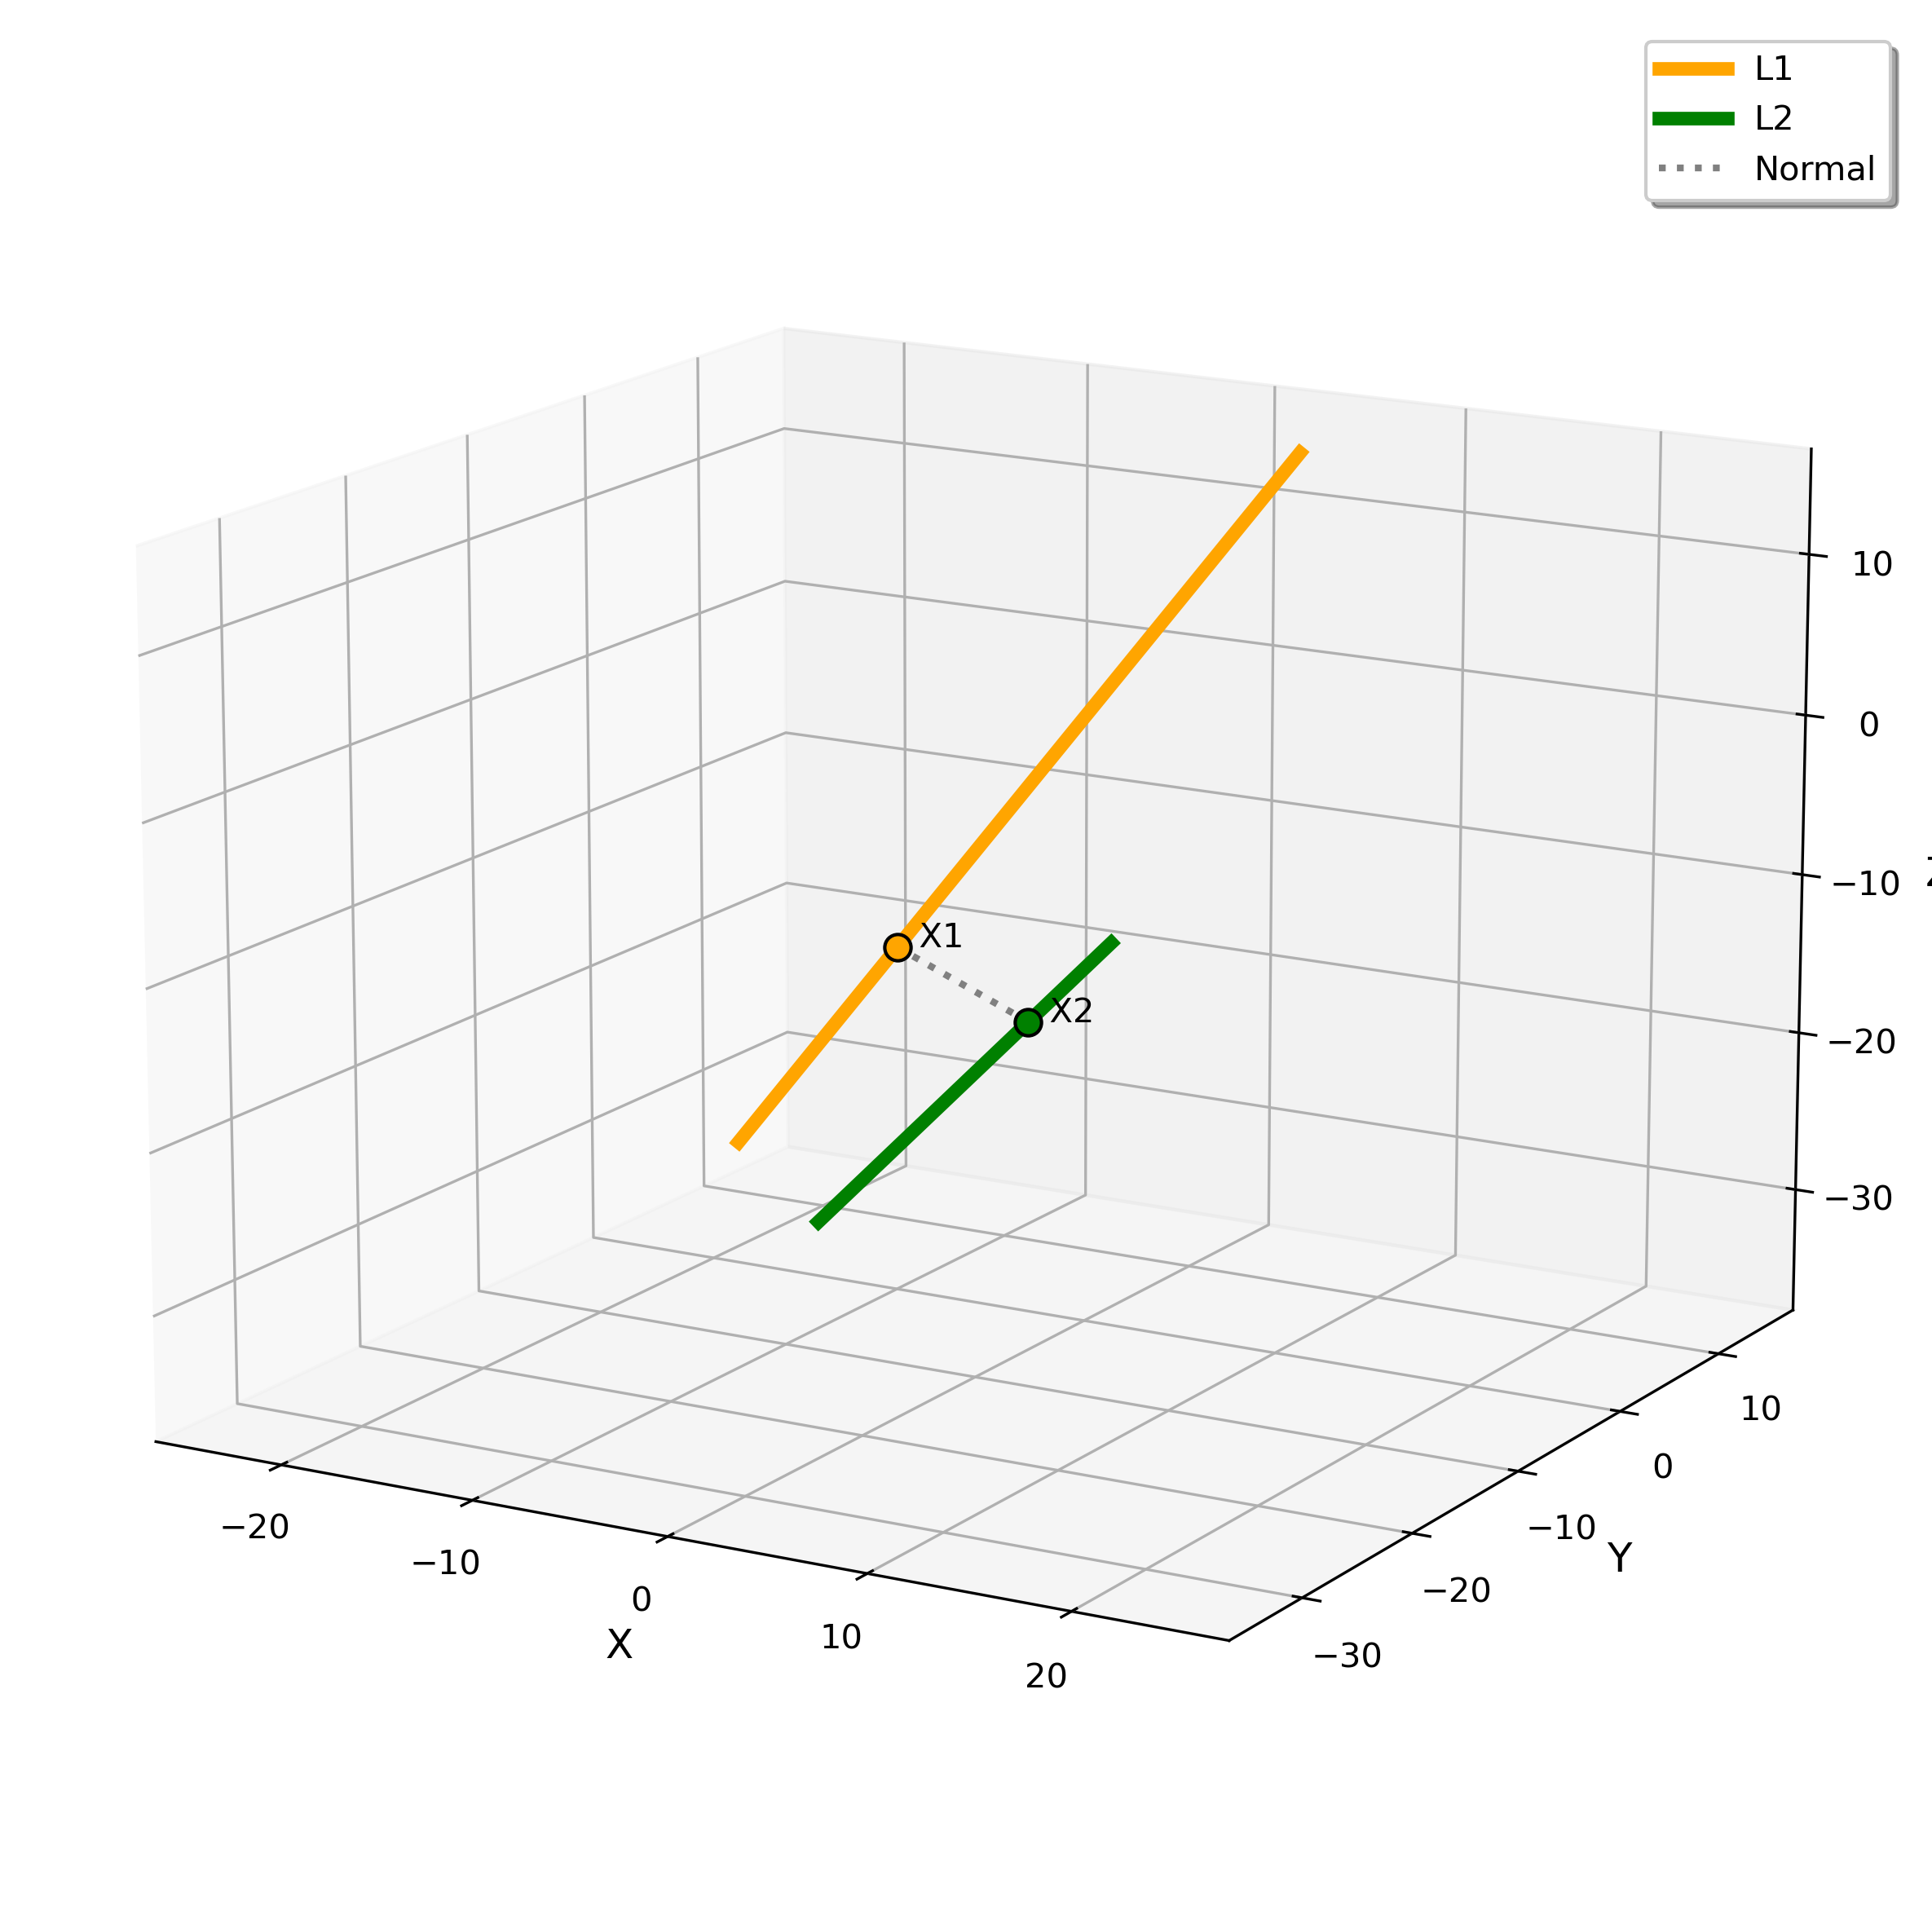
\includegraphics[width=\columnwidth]{figs/fig1.png}
    \caption{Skew Lines}
    \label{fig:fig/fig1.png}
\end{figure}
\end{document}  
